\documentclass[12pt]{report}
\usepackage{graphicx}
\usepackage{scribe_MG}
\usepackage{amssymb}
\usepackage{graphicx}
\usepackage[mathscr]{eucal}
\usepackage[english]{babel}
\usepackage[utf8]{inputenc}  %encodage du fichier
\usepackage[T1]{fontenc}
\usepackage{epstopdf}
\usepackage{tikz}
\usepackage{array}

\usepackage{placeins}

\newcommand\independent{\protect\mathpalette{\protect\independenT}{\perp}}
\def\independenT#1#2{\mathrel{\rlap{$#1#2$}\mkern2mu{#1#2}}} 

\newcommand{\indep}{\ensuremath{\,\bot\!\!\!\bot\,}} %% The symbol for independent
\newcommand{\notindep}{\indep\!\!\!\!\!/\,\,\,}

\newtheorem{remark}{Remark}[section]
\newtheorem{example}{Example}[section]
\newtheorem{property}{Property}[section]


\begin{document}
\coursetitle{Directed and Undirected Graphs}
\semester{2013/2014}
\lecturer{Francis Bach} \scribe{Vincent Bodin, Thomas Moreau}
\lecturenumber{4} \lecturedate{October 23rd}

\maketitle


%% Vincent

\section{Notation and probability recalls}


Let us recall a few notations before establishing some properties of directed graphical model. Let $X_1, X_2, \cdots, X_n$ be random variables of law: 
\begin{equation*}
\mathbb{P}(X_1 = x_1, X_2 = x_2, \cdots, X_n = x_n) = p_X (x_1, \cdots, x_n) = p(x)
\end{equation*}
where $x$ stands for $(x_1, \cdots, x_n)$. Given $A\subset \{1, \cdots, n\}$, we denote the marginal law of $x$ according to $A$ by: 
\begin{equation*}
p(x_A) = \sum_{x\in {A^c}} p(x_A, x_{A^c})
\end{equation*}
With this notation we can write the conditional law as: 
\begin{equation*}
p( x_A | x_{A^c} ) = \frac{p(x_A, x_{A^c})}{p(x_{A^c})}
\end{equation*}
We also recall the so-called 'chain rule' stating:
\begin{equation*}
p(x_1, \cdots, x_n) = p(x_1) p(x_2 | x_1) p(x_3 | x_2, x_1) \cdots p(x_n | x_1, \cdots, x_{n-1})
\end{equation*}
To end with notations and recalls, we remind the conditional independence: 
\begin{equation*}
X\indep Y \ | \ Z \Leftrightarrow p\left(x,y|z\right)=p\left(x|z\right)p\left(y|z\right) \Leftrightarrow p\left(x|y,z\right)=p\left(x|z\right)=\frac{p\left(x,y|z\right)}{p\left(y|z\right)}
\end{equation*}





\section{Directed Graphical Model}

\subsection{First definitions and properties}

Let $X_1, \cdots, X_n$ be $n$ random variables of law $p(x) = p_X (x_1, \cdots, x_n)$. 
\begin{definition}
Let $G = (V,E)$ be a DAG with $V = \{1,\cdots, n\}$. We say that $p(x)$ factorizes in G, noted $p(x)\in \mathcal{L}(G)$ if $p(x)$ is of the form:
\begin{equation}
\forall x, p(x) = \prod_{i=1}^n f_i(x_i, x_{\pi_i}) \text{ such that } f_i\geq 0, \sum_{x_i} f(x_i, x_{\pi_i}) = 1
\end{equation}
where we recall that $\pi_i$ stands for the set of parents of the vertex $i$ in $G$.
\end{definition}

We now show that because we assumed that G was a DAG, it implies a particular and convenient form for the $f_i$ above. We have: 

\begin{proposition}
If $p(x)\in\mathcal{L}(G)$ then, for all $i\in\{1,\cdots,n\}$, $f_i(x_i, x_{\pi_i}) = p(x_i | x_{\pi_i})$.
\end{proposition}
\begin{proof}
We prove this by induction on $n = |V|$ cardinal of the set $V$. Since $G$ is a DAG, there exists a leaf, \emph{i.e.} a node with no children. Without lost of generality, we can assume that the leaf is labeled by $n$. We first notice: 
\begin{equation}
\begin{array}{r l l}
	\forall x, p(x_1, \cdots, x_{n-1}) & = & \displaystyle\sum_{x_n} p(x_1, \cdots, x_n) \\
																		 & = & \displaystyle\sum_{x_n} \prod_{i=1}^{n} f_i(x_i,x_{\pi_i}) \\
																		 & = & \displaystyle\sum_{x_n} f_n(x_n, x_{\pi_n})\prod_{i=1}^{n-1} f_i(x_i,x_{\pi_i}) \\
																		 & = & \displaystyle\prod_{i=1}^{n-1} f_i(x_i,x_{\pi_i}) \sum_{x_n} f_n(x_n, x_{\pi_n}) \hspace{0.2cm} (*)  \\
																		 & = & \displaystyle\prod_{i=1}^{n-1} f_i(x_i,x_{\pi_i}) \\
																		 & = & \displaystyle g(x_1, \cdots, x_{n-1}) \hspace{0.2cm} (**)
\end{array}
\label{eq:}
\end{equation}
The step $(*)$ is justified by the fact that $n$ is a leaf and thus it never appears in any of the $\pi_i$ for $i\in\{1,\cdots,n-1\}$. Step $(**)$ is also justified by the same kind of reasoning: since $n$ is a leaf it cannot appear in any of the $\pi_i$ explaining why it is only a function, say $g$, of $x_1,\cdots, x_{n-1}$. From this result, we can use an induction reasoning noticing that $G - \{n\}$ is still a DAG. To conclude this proof, we simply need to show that, indeed, $f_n(x_n, x_{\pi_n}) = p(x_n | x_{\pi_n})$ - this property will automatically propagates by induction. We have: 
\begin{equation}
p(x_n, x_{\pi_n}) = \sum_{x_i, i\notin \{n\}\cup \pi_n} p(x) = \left( \sum_{x_i, i\notin \{n\}\cup \pi_n} g(x_1, \cdots, g_{n-1})\right)f_n(x_n, x_{\pi_n})
\label{eq:}
\end{equation}
Noticing that $\sum_{x_i, i\notin \{n\}\cup \pi_n} g(x_1, \cdots, x_{n-1})$ is a function of only $x_{\pi_n}$, say $h(x_{\pi_n})$, we can derive: 
\begin{equation}
p(x_n | x_{\pi_n}) = \frac{p(x_n, x_{\pi_n})}{\sum_{x'_n}p(x'_n, x_{\pi_n})} = \frac{h(x_{\pi_n}) f_n(x_n, x_{\pi_n})}{h(x_{\pi_n})} = f_n(x_n, x_{\pi_n})
\label{eq:}
\end{equation}
\end{proof}

Hence we can give an equivalent definition for a DAG to the notion of factorizing: 

\begin{definition}
(Equivalent definition) $p(x)$ factorizes in $G$, noted $p(x)\in \mathcal{L}(G)$ if:
\begin{equation}
\forall x, p(x) = \prod_{i=1}^n p(x_i | x_{\pi_i})
\label{eq:}
\end{equation}
\end{definition}


\begin{example}
\begin{itemize}
	\item (Trivial Graphs) Assume $E = \emptyset$, \emph{i.e.} there is no edges. Then we have $p(x) = \prod_{i=1}^n p(x_i)$, implying the random variables $X_1, \cdots, X_n$ are independent. Hence variables are independent if they factorize in the empty graph. 
	\item (Complete Graphs) Assume now we have a complete graph (thus with $n(n-1)/2$ edges as we need acyclic for it to be a DAG), we have: $p(x) = \prod_{i=1}^n p(x_i | x_1, \cdots, x_{i-1})$, the so-called 'chain rule' which is always true. Every random process factorizes in the complete graph.
\end{itemize}
\end{example}



\subsection{Graphs with three nodes}

We give an insight of the different possible behaviors of a graph by thoroughly enumerating the possibilities for a 3-nodes graph. 
\begin{itemize}
	\item The two first options are the empty graph, leading to independence, and the complete graph that gives no further information than the chain rule.
	
	\item (Markov chain) A Markov chain is a certain type of DAG showed in Fig.(\ref{fig1}). In this configuration we show that we have:
	\begin{equation}
		p(x,y,z) \in \mathcal{L}(G) \Rightarrow X \indep Z\ |\ Y
	\label{eq:}
	\end{equation}
	Indeed we have:
	\begin{equation*}
	p(z|y,x) = \frac{p(x,y,z)}{p(x,y)} = \frac{p(x,y,z)}{\sum_{z'} p(z',x,y)} = \frac{p(x) p(y|x) p(z|y)}{\sum_{z'}p(x) p(y|x) p(z'|y)} = p(z|y)
	\end{equation*}
	\begin{figure}[h!]
		\centering
			\includegraphics[scale=.75]{fig1.eps}
		\caption{Markov Chain}\label{fig1}
	\end{figure}
	
	\item (Latent cause) It is the type of DAG given in Fig.(\ref{fig2}). We show that:
	\begin{equation}
		p(x) \in \mathcal{L}(G) \Rightarrow X \indep Y\ |\ Z
	\label{eq:}
	\end{equation}
	Indeed:
	\begin{equation*}
	p(x,y|z) \frac{p(x,y,z)}{p(z)} = \frac{p(z)p(y|z)p(x|z)}{p(z)} = p(x|z)p(y|z)
	\end{equation*}
	\begin{figure}[h!]
	\centering
	\includegraphics[scale=.75]{fig2.eps}
	\caption{Latent cause}
	\label{fig2}
	\end{figure}
	
	\item (Explaining away) Represented in Fig.(\ref{fig3}), we can show for this type of graph:
	\begin{equation}
	 p(x) \in\mathcal{L}(G) \Rightarrow X\indep Y
	\label{eq:}
	\end{equation}
	It basically stems from:
	\begin{equation*}
		p(x,y) = \sum_z p(x,y,z) = p(x)p(y) \sum_z p(z) = p(x) p(y)
	\end{equation*}
	\begin{figure}[h!]
	\centering
	\includegraphics[scale=.75]{fig3.eps}
	\caption{Explaining away}
	\label{fig3}
	\end{figure}
\end{itemize}


\begin{remark}
The use of 'cause' is not advised since statistics provide with correlations and no causality notion. Note also that in the 'explaining away' graph, in general $X\indep Y | Z$ is not true. Last, it is important to figure that not every relationships can be expressed in terms of graphical modes. As a counter-example take three random variables pairwise independent, but not fully independent. 
\end{remark}


\subsection{Inclusion, reversal and marginalization properties}

\hspace{.5cm}\textbf{Inclusion property. }Here is a quite intuitive proposition about included graphs and their factorization.
\begin{proposition}
If $G = (V,E)$ and $G' = (V,E')$ then: 
\begin{equation}
E \subset E' \Leftrightarrow \mathcal{L}(G) \subset \mathcal{L}(G)
\label{eq:}
\end{equation}
\end{proposition}
\begin{proof}
We have $p(x) = \prod_{i=1}^n p(x_i, x_{\pi_i(G)})$. As $E \subset E'$ it is obvious that $\pi_i(G) \subset \pi_i(G')$, then we have: $p(x) = \prod_{i=1}^n p(x_i, x_{\pi_i(G')})$, proving that $p(x)$ factorizes in $G'$ as well.
\end{proof}

\textbf{Reversal property. }We also have some reversal properties. Let us first define the notion of V-structure.
\begin{definition}
We say there is a V-structure in $i\in V$ if $| \pi_i|\geq 2$, \ie $i$ has two or more parents.
\end{definition}
\begin{figure}[h!]
\centering
\includegraphics[scale = 1]{vstruct.eps}
\caption{V-structure}
\label{fig4}
\end{figure}
\begin{proposition}
(Markov equivalence) If $G = (V,E)$ is a DAG and if for $(i,j)\in E, | \pi_i| = 0$ and $|\pi_j| \leq 1$, then $(i,j)$ may be reversed, \emph{i.e.} if $p(x)$ factorizes in $G$ then it factorizes in $G' = (V,E')$ with $E' = (E-\{(i,j)\})\cup \{ (j,i)\}$.
\end{proposition}
In terms of 3-nodes graph, this property ensures us that the Markov chain and latent cause are equivalent. On the other hand the V-structure is a different class of graph compared to the two others.
\begin{definition}
An edge $(i,j)$ is said to be covered if $\pi_j = \{i \}\cup \pi_i$. 
\end{definition}
By reversing $(i,j)$ we might not get a DAG as it might break the acyclic property. We have the following result:
\begin{proposition}
Let $G = (V,E)$ be a graph and $(i,j)\in E$ a covered edge. Let $G'= (V,E')$ with $E' = (E-\{(i,j)\})\cup \{ (j,i)\}$, then if $G'$ is a DAG, $\mathcal{L}(G) = \mathcal{L}(G')$.
\end{proposition}

\textbf{Marginalization. }The underlying question is to know which kind of graphs can be factorized in a sub-graph. It might not be true in general, but we show that as long we marginalize by removing a leaf it is. 
\begin{proposition}
If $i$ is a leaf, then $p(x_j, j \neq i)$ factorizes in the sub-graph obtained by removing the leaf $i$.
\end{proposition}
\begin{proof}
It is simply derived by the following computation:
\begin{equation*}
\begin{array}{r l l}
   p(x_1,...x_{n-1}) & = & \displaystyle \sum_{x_n}{p(x_1,\ldots,x_n)}\\
                     & = & \displaystyle \sum_{x_n}{\left(\prod_{i=1}^{n-1}{p(x_{i}|x_{\pi_i})} p(x_n|x_{\pi_n})\right)}\\
										 & = & \displaystyle \prod_{i=1}^{n-1}{p(x_{i}|x_{\pi_i})}\sum_{x_n}{p(x_n|x_{\pi_n})}\\
                     & = & \displaystyle \prod_{i=1}^{n-1}{p(x_{i}|x_{\pi_i})}
\end{array}
\end{equation*}
\end{proof}

\textbf{Conditional independence. }We finish this section by giving a result that explains that if $p(x)$ factorizes in $G$ then every single random variable is independent to the set of its non-descendants conditionally to the knowledge of its parents. From now on, we denote by $\text{nd}(i)$ the set of non-descendants of $i$.

\begin{proposition}
If $G$ is a DAG, then: 
\begin{equation}
p(x) \in \mathcal{L}(G) \Leftrightarrow X_i \indep X_{\text{nd}(i)} | X_{\pi_i}
\end{equation}
\end{proposition}
\begin{proof}
We will only prove the $\Rightarrow$ way. Assume $(1,\cdots, n)$ is a topological order then: 
\begin{equation*}
\left\{
\begin{array}{r l l l}
p(x) & = & \displaystyle \prod_{i=1}^n p(x_i | x_{\pi_i}) & \text{ : because $p(x)\in\mathcal{L}(G)$} \\
p(x) & = & \displaystyle \prod_{i=1}^n p(x_i | x_1, \cdots, x_{i-1}) & \text{ : chain rule, always true} \\
\end{array}
\right.
\end{equation*}
As we chose a topological order, we have $\pi_i \subset \{1, \cdots, i-1 \}$, and we show by induction that:
\begin{equation*}
p(x_i | x_{\pi_i}) = p(x_i | x_1, \cdots, x_{i-1}) = p(x_i | x_{\pi_i}, x_{\{ 1,\cdots, i-1\} - \pi_i})
\end{equation*}
This directly implies that $X_i \indep X_{\pi_i - \{ 1,\cdots, i-1\}} | X_{\pi_i}$. The key idea now is to notice that for all $i$, there exist a topological order such that $\text{nd}(i) \subset \{1,\cdots, i-1\}$.
\end{proof}




\subsection{d-separation}

We want to answer queries such as, given $A, B$ and $C$ three subsets, is $X_A \indep X_B | X_c$ true? To answer those issues we need the d-separation notion, terminology standing for directed separation. Indeed it is easy to figure out that the notion of separation is not enough in a directed graph and needs to be generalized. 

\begin{definition}
Let $a,b\in V$, a chain from $a$ to $b$ is a sequence of nodes, say $(v_1, \cdots, v_n)$ such that $v_1 = a$ and $v_n = b$ and $\forall j, (v_j, v_{j+1}) \in E$ or $(v_j, v_{j+1}) \in E$.
\end{definition}

We can notice that a chain is hence a path in the symmetrized graph, \emph{i.e.} in the graph where if the relation $\rightarrow$ is true then $\leftrightarrow$ is true as well. Assume $C$ is a set that is observed. We want to define a notion of being 'blocked' by this set $C$ in order to answer the underlying question above. 

\begin{definition}
\begin{enumerate}
\item A chain from $a$ et $b$ is blocked in $d$ if:
\begin{itemize}
\item either $d\in C$ and $(v_{i-1}, v_i, v_{i+1})$ is not a V-structure;
\item or $d\notin C$ and $(v_{i-1}, v_i, v_{i+1})$ is a V-structure and no descendants of $d$ is in C.
\end{itemize}

\item A chain from $a$ to $b$ is blocked if and only if it is blocked at any nodes.

\item $A$ and $B$ are said to be d-separated by $C$ if and only if all chains that go from $a\in A$ to $b\in B$.
\end{enumerate}
\end{definition}


\begin{example}
\begin{itemize}
\item (Markov chain) If you try to prove that any set of the future is independent to the past given the present with Markov theory, it might be painful but the d-separation notion gives the results directly.
\begin{figure}[h!]
\centering
	\includegraphics[scale=1]{markov.eps}
\caption{Markov chain}
\end{figure}

\item (Hidden Markov Model) Often used because we only observe a noisy observation of the random process.
\begin{figure}[h!]
\begin{center}
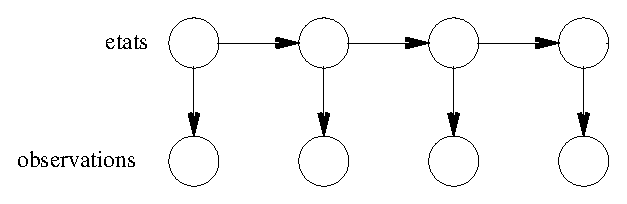
\includegraphics[scale=1]{hmm.eps}
\end{center}
\caption{Hidden Markov Model}
\end{figure}
\end{itemize}
\end{example}











%% Thomas

\section{Undirected graphical models}

\subsection{Definition}

\begin{definition}
Let $G = (V, E)$ be a \emph{\textbf{undirected graph}}. We denote by $\mathcal{C}$ a set of cliques of $G$ \ie a set of sets of fully connected vertices. We say that a probability distribution $p$ factorizes in G and denote $p \in \mathcal{L}(G)$ if p(x) is of the form:
\begin{equation*}
p(x) = \frac{1}{Z} \prod_{C \in \mathcal{C}} \psi_C(x_C) \text{ with } \psi_C \geq 0, Z = \sum_{x}\prod_{C \in \mathcal{C}} \psi_C(x_C)
\end{equation*}
\end{definition}

\begin{danger}
The functions $\psi_C$ are not probability distributions like in the directed graphical models. They are called potentials.
\end{danger}

\begin{remark}
With the normalization by $Z$ of this expression, we see that the function $\psi_C$ are defined up to a multiplicative constant.
\end{remark}
\begin{remark}
We may restrict $\mathcal{C}$ to $\mathcal{C}_{max}$, the set of maximal cliques.
\end{remark}
\begin{remark}
This definition can be extended to any function: $f$ is said to factorize in $G \iff f(x) = \prod_{C \in \mathcal{C}} \psi_C(x_C)$.
\end{remark}


\subsection{Trivial graphs}

\begin{tabular}{c p{11cm}}
\textbf{Empty graphs}  & We consider $G = (V, E)$ with $E = \emptyset$. For $p \in \mathcal{L}(G)$, we get: 
\begin{equation*}
p(x) = \prod_{i=1}^n \psi_i(x_i) \text{ as } \mathcal{C} = \{ \{i\}\in V\}
\end{equation*}
This gives us that $X_1, ..., X_n$ are mutually independent.\\
	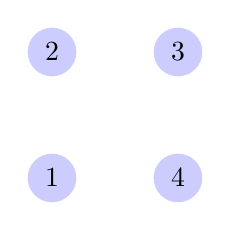
\begin{tikzpicture}
		  [scale=.8,auto=left,every node/.style={circle,fill=blue!20}]
		  \node (n1) at (1,1) {1};
		  \node (n2) at (1,3)  {2};
		  \node (n3) at (3,3)  {3};
		  \node (n4) at (3,1) {4};
	\end{tikzpicture} & \\
\end{tabular}

\begin{tabular}{c p{11cm}}
\textbf{Complete graphs} & We consider $G = (V, E)$ with $\forall i, j \in V, (i,j) \in E$. For $p \in \mathcal{L}(G)$, we get: 
\begin{equation*}
p(x) = \frac{1}{Z} \psi_V(x_V) \text{ as } \mathcal{C} \text{ is reduced to a single set V}
\end{equation*}
This gives no further information upon the n-sample $X_1, ..., X_n$.\\
	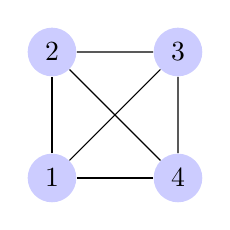
\begin{tikzpicture}
		[scale=.8,auto=left,every node/.style={circle,fill=blue!20}]
		\node (n1) at (1,1) {1};
		\node (n2) at (1,3)  {2};
		\node (n3) at (3,3)  {3};
		\node (n4) at (3,1) {4};
		\foreach \from/\to in {n1/n2,n2/n3,n3/n4,n4/n1, n1/n3, n2/n4}
			\draw (\from) -- (\to);
	\end{tikzpicture}
\end{tabular}

\subsection{Separation and conditional dependence}

\begin{proposition}
Let $G = (V, E)$ and $G' = (V, E')$ be 2 undirected graph.\\
\begin{equation*}
E \subseteq E' \Rightarrow \mathcal{L}(G) \subseteq \mathcal{L}(G')
\end{equation*}
\end{proposition}

\begin{definition}
We say that $p$ satisfies the \emph{\textbf{Global Markov property}} w.r.t. $G$ if and only if for all $A, B, S \subset V$ disjoint subsets: A and B are separated by $S \Rightarrow X_A \indep X_B | X_S$.
\end{definition}

\begin{proposition}
If $p \in \mathcal{L}(G) $ then, $p$ satisfies the Global Markov property w.r.t. $G$.\\
\end{proposition}

\begin{proof}
We can consider that $A\cup B\cup S = V$ without loss of generality as we could replace $A$ and $B$ by :\\
\centerline{
\begin{tabular}{c l}
&$\widetilde{A} = A \cup \{a \in V$  / a and A are not separated by S \}\\
&$\widetilde{B} = V\setminus \{S \cup \widetilde{A}\}$
\end{tabular}
}
$\widetilde{A}$ and $\widetilde{B}$ are separated by S.

We consider $C \in \mathcal{C}$. It is not possible to have $C \cap A \neq \emptyset$ and $C \cap B \neq \emptyset$ as A and B are separated by S. Then $C \subset A \cup S$ or $C \subset B \cup S$.
\begin{equation*}
p(x) =  \displaystyle \frac{1}{Z} \prod_{C \in \mathcal{C} \atop C \in A \cup S} \psi_C(x_C) \prod_{C \in \mathcal{C} \atop C \in B \cup S} \psi_C(x_C) = f(x_{A \cup S}) g(x_{B \cup S})
\end{equation*}

\centerline{\begin{tabular}{r c c c c}
$p(x_A| x_S, x_B)$ & = &  $\displaystyle \frac{p(x_A, x_B, x_S)}{p(x_S, x_B)}$ & = & $\displaystyle \frac{f(x_A, x_S)g(x_S,w_B)}{\sum_{x_{A}^{'}} f(x_{A}^{'}, x_S) g(x_B, x_S)}$ \\
&&&=& $\displaystyle \frac{f(x_A, x_S)}{\sum_{x_{A}^{'}} f(x_{A}^{'}, x_S)}$\\
&&&=& $p(x_A| x_S)$ \\
\end{tabular}}
Thus, $X_A \indep X_B | X_S$
\end{proof}

\begin{theorem} 
(Hammersley - Clifford) If $\forall x, p(x) > 0$ then $p \in \mathcal{L}(G) \iff $ p satisfies the global Markov property.
\end{theorem}

\subsection{Marginalization}

As for directed graph, we also have a marginalization notion in undirected graphs. We see still that it is slightly different since we need to marginalize not only by a leaf in undirected graphs but by all the neighbors.
\begin{definition}
For $i \in V$, the \emph{\textbf{Markov blanket}} is the smallest set of nodes that makes $X_i$ independent to the rest of the graph.
\end{definition}

\begin{remark}
The Markov blanket in an undirected graph for $i \in V$ is the set of its neighbors.
\end{remark}

\begin{proposition}
Let $G = (V, E)$ be an undirected graph and $G' = (V', E')$ the graph obtain for $V' = V \setminus \{n\}$ and $E'$ the set of edge connecting all the neighbors of n. If $p \in \mathcal{L}(G)$ then $p(x_1, ..., x_{n-1}) \in \mathcal{L}(G')$.
\end{proposition}

\subsection{Relation between directed and undirected graphical models}

Since now we have seen that many notions developed for directed graph naturally extended to undirected graphs. The raising question is thus to know whether we can find a theory including both directed and undirected graphs, in particular, is there a way - for instance by symmetrizing the directed graph as we have done repeatedly - to find a general equivalence between those two notions. The answer is no, as we will discuss - though it might work in some special cases described above.
\begin{center}
	\begin{tabular}{|c|c|c|}
  	\hline
      & Directed graphical model    & Undirected graphical model \\\hline
      Factorization      & $p(x)=\displaystyle\prod_{i=1}^{n}p(x_i|x_{\pi_i})$ &
      $p(x)=\frac{1}{Z}\displaystyle\prod_{C\in\mathcal{C}}\psi_C(x_C)$ \\\hline
      Set independence       & d-separation  & separation \\\hline
      Marginalization       & non close  & close \\\hline
      Not equivalent&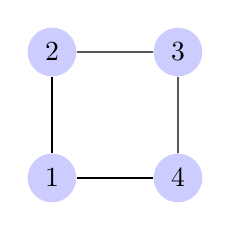
\begin{tikzpicture}
		  [scale=.8,auto=left,every node/.style={circle,fill=blue!20}]
		  \node (n1) at (1,1) {1};
		  \node (n2) at (1,3)  {2};
		  \node (n3) at (3,3)  {3};
		  \node (n4) at (3,1) {4};
		  \foreach \from/\to in {n1/n2,n2/n3,n3/n4,n4/n1}
			\draw (\from) --  (\to);
		\end{tikzpicture} 
		&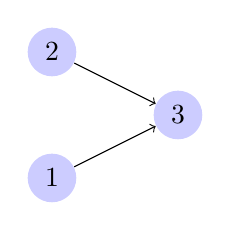
\begin{tikzpicture}
		  [scale=.8,auto=left,every node/.style={circle,fill=blue!20}]
		  \node (n1) at (1,1) {1};
		  \node (n2) at (1,3)  {2};
		  \node (n3) at (3,2)  {3};
		  \foreach \from/\to in {n1/n3,n2/n3}
			\draw[->] (\from) --  (\to);
		\end{tikzpicture} \\\hline
   \end{tabular}
\end{center}

Let $G$ be DAG. Can we find $G'$ undirected such that $\mathcal{L}(G) = \mathcal{L}(G')$? $\mathcal{L}(G) \subset \mathcal{L}(G')$?

\begin{definition}
	Let $G=(V,E)$ be a \emph{DAG}. The \emph{\textbf{symmetrized graph}} of $G$ is $\tilde{G}=(V,\tilde{E})$, with $\tilde E = \{(u,v), (v, u) / (u,v) \in E\}$.
\end{definition}

\begin{definition}
	Let $G=(V,E)$ be a \emph{DAG}. The \emph{\textbf{moralized graph}} $\bar{G}$ of $G$ is the symmetrized graph $\tilde{G}$, where we add edge such that for all $v \in V$, $\pi_v$ is a clique.
\end{definition}

We admit the following proposition:
\begin{proposition}
	Let $G$ be a \emph{DAG} without any V-structure, then $\bar{G} = \tilde{G}$ and $\mathcal{L}(G)=\mathcal{L}(\tilde{G})=\mathcal{L}(\bar{G}).$
\end{proposition}
In case there is a V-structure in the graph, we can only conclude:
\begin{proposition}
	Let $G$ be a \emph{DAG}, then $\mathcal{L}(G) \subset \mathcal{L}(\bar{G})$.
\end{proposition}
$\bar{G}$ is minimal for the number of edges in the set $H$ of undirected graphs such that $\mathcal{L}(G)\subset\mathcal{L}(H)$.
\begin{danger} Not all conditional independence structure for random variable can be factorized in a graphical model (directed or undirected).
\end{danger}



\end{document}
